\documentclass[twoside]{article}
\setlength{\oddsidemargin}{0.25 in}
\setlength{\evensidemargin}{-0.25 in}
\setlength{\topmargin}{-0.6 in}
\setlength{\textwidth}{6.5 in}
\setlength{\textheight}{8.5 in}
\setlength{\headsep}{0.75 in}
\setlength{\parindent}{0 in}
\setlength{\parskip}{0.1 in}

%
% ADD PACKAGES here:
%

\usepackage{amsmath,amsfonts,amssymb,graphicx,mathtools,flexisym}
\usepackage[framemethod=TikZ]{mdframed}
\usepackage[utf8]{inputenc}
\usepackage{cancel}
\usepackage{pgfplots}
\usepackage{multicol}
\usepackage{enumitem}

%
% Theorem style
%
\mdfdefinestyle{minimal}{
	topline		= false,
	rightline	= false,
	bottomline	= false,
	leftline	= false
}

\mdfdefinestyle{left}{
	topline		=false,
	rightline	=false,
	bottomline	=false
}

\mdfdefinestyle{frame}{
	topline		= true,
	rightline	= true,
	bottomline	= true,
	leftline	= true,
	shadow		= false
}

\newmdenv[style=left,frametitle=Definition]{definition}
\newmdenv[style=minimal,frametitle=Beispiel]{expl}
%\newmdenv[style=frame,frametitle={\colorbox{white}{\space Lemma\space}},
%    innertopmargin=0pt,
%    frametitleaboveskip=-\ht\strutbox,]{lemma}
\newmdenv[style=frame,frametitle=Satz]{satz}
\newmdenv[style=minimal,frametitle=Beweis]{proof}
\newenvironment{lemma}[1][]{%
  \ifstrempty{#1}%
  {
	\mdfsetup{frametitle={\colorbox{white}{\space Lemma\space}};}
  }
  {
	\mdfsetup{frametitle={\colorbox{white}{\space Lemma #1\space}};}
  }
  \mdfsetup{style=frame,innertopmargin=0pt,%
            linewidth=1pt,%
            frametitleaboveskip=-\ht\strutbox,}
  \begin{mdframed}[]\relax%
  }{\end{mdframed}}

%
% The following commands set up the lecnum (lecture number)
% counter and make various numbering schemes work relative
% to the lecture number.
%
\newcounter{lecnum}
\renewcommand{\thepage}{\thelecnum-\arabic{page}}
\renewcommand{\thesection}{\arabic{section}}
\renewcommand{\theequation}{\thesection.\arabic{equation}}
\renewcommand{\thefigure}{\thesection.\arabic{figure}}
\renewcommand{\thetable}{\thesection.\arabic{table}}

%
% The following macro is used to generate the header.
%
\newcommand{\lecture}[4]{
   \pagestyle{myheadings}
   %\thispagestyle{plain}
   \newpage
   \setcounter{lecnum}{#1}
   \setcounter{page}{1}
   \noindent
   \begin{center}
   \framebox{
      \vbox{\vspace{2mm}
    \hbox to 6.28in { {\bf DGL IIa
    \hfill SoSe 2017} }
       \vspace{4mm}
       \hbox to 6.28in { {\Large \hfill Vorlesung #1: #2  \hfill} }
       \vspace{2mm}
       \hbox to 6.28in { {\it Dozent: #3 \hfill Mitschrift: #4} }
      \vspace{2mm}}
   }
   \end{center}
   \markboth{Vorlesung #1: #2}{Vorlesung #1: #2}

   \vspace*{4mm}
}
%
% Convention for citations is authors' initials followed by the year.
% For example, to cite a paper by Leighton and Maggs you would type
% \cite{LM89}, and to cite a paper by Strassen you would type \cite{S69}.
% (To avoid bibliography problems, for now we redefine the \cite command.)
% Also commands that create a suitable format for the reference list.
\renewcommand{\cite}[1]{[#1]}
\def\beginrefs{\begin{list}%
        {[\arabic{equation}]}{\usecounter{equation}
         \setlength{\leftmargin}{2.0truecm}\setlength{\labelsep}{0.4truecm}%
         \setlength{\labelwidth}{1.6truecm}}}
\def\endrefs{\end{list}}
\def\bibentry#1{\item[\hbox{[#1]}]}

%Use this command for a figure; it puts a figure in wherever you want it.
%usage: \fig{NUMBER}{SPACE-IN-INCHES}{CAPTION}
\newcommand{\fig}[3]{
            \vspace{#2}
            \begin{center}
            Figure \thelecnum.#1:~#3
            \end{center}
    }
% Use these for theorems, lemmas, proofs, etc.

% **** IF YOU WANT TO DEFINE ADDITIONAL MACROS FOR YOURSELF, PUT THEM HERE:

\def\R{\mathbb{R}}      	% The reals
\def\C{\mathcal{C}}     	% continuous functions
\def\W{\Omega}          	% Capital omega
\def\w{\omega}          	% Lowercase omega
\def\L{\mathrm{L}}	     	% Lebesgue-integrable functions
\def\esssup{\text{ess sup}} % Essential supremum
\def\iff{\Leftrightarrow}   % If and only if
\def\implies{\Rightarrow}   % Implies
\def\e{\epsilon}            % Epsilon
\def\d{\delta}              % Delta

% changed commands

\renewcommand*\labelitemi{\normalfont\bfseries\textendash}
\setlist[itemize]{noitemsep, topsep=-8pt}

\begin{document}
%\lecture{**LECTURE-NUMBER**}{**DATE**}{**LECTURER**}{**SCRIBE**}
%\footnotetext{These notes are partially based on those of Nigel Mansell.}

% **** YOUR NOTES GO HERE:
\lecture{1}{18.04.2017}{Dr. Raphael Kruse}{Frank Rehfeld}
\section{Verallgemeinerte Ableitungen im Eindimensionalen}

\textbf{Motivation}\\
$u\colon\W\to\R$ gesucht mit
\begin{align*}
	-&u^{\prime\prime}\left(x\right) = f\left(x\right) \forall x\in\Omega\\
	 &u\left(a\right) = u\left(b\right) = 0 \forall x\in\partial\Omega
\end{align*}
für ein gegebenes $f$

\textbf{Ziel}\\
Lösungsbegriff abschwächen um unstetige $f$ umzusetzen. Idee hierfür ist die Multiplikation mit Testfunktionen und anschließende partielle Integration.
\begin{equation*}
	\int_{a}^{b} u^{\prime}\left(x\right)v^{\prime}\left(x\right) + \cancel{\left[u^{\prime}\left(x\right)v\left(x\right)\right]_{a}^{b}} = \int_{a}^{b} f\left(x\right)v\left(x\right)
\end{equation*}
Somit ist nicht mehr nötig, dass $u\in\C^{2}$. Dafür zusätzliche Forderung: $u^{\prime}v^{\prime}, fv\in\L^{1}$

\lecture{2}{19.04.2017}{Dr. Raphael Kruse}{Frank Rehfeld}
\textbf{Wiederholung}\\
\begin{enumerate}
\item	
	$\begin{cases}
			u\colon\W=\left(a,b\right)\to\R\\
			\int_{\W}u^{\prime}\left(x\right)v^{\prime}\left(x\right)\,\mathrm{d}x = \int_{\W}f\left(x\right)v\left(x\right)\,\mathrm{d}x\\
			u\left(a\right)=u\left(b\right)
		\end{cases}$
\item{}
	Eigenschaften $\L^{p}$:\\
	\begin{itemize}
		\item $1\leq p <\infty \implies \L^{p}\text{ separabel}$
		\item $\L^{\infty}$ nicht separabel
		\item $1 < p <\infty, \frac{1}{p}+\frac{1}{q}=1 \implies \left(\L^{p}\right)^{\prime} \equiv \L^{q}$\\
			  $T\colon \L^{q}\to\left(\L^{p}\right)^{\prime}, \left(Tg\right)f = \int_{\W}f\left(x\right)g\left(x\right)\,\mathrm{d}x$
		\item $\left(\L^{1}\right)^{\prime}\equiv\L^{\infty}, \L^{1}\subsetneq\left(\L^{\infty}\right)^{\prime}$\\
				$\implies \L^{1}, \L^{\infty}$ sind nicht reflexiv
	\end{itemize}
\end{enumerate}

\begin{definition}
	$\L^{1}_{\text{loc}}\left(\W\right) := \left\{u\colon\W\to\R\colon u|_{K}\in\L^{1}\left(K\right)\forall K\subset\W \text{ kompakt}\right\}$\\
	Raum der lokal integrierbaren Abbildungen
\end{definition}

\begin{definition}
	$\C^{\infty}_{\text{c}}\left(\W\right) := \left\{f\colon\W\to\R\colon f\in\C^{\infty},\operatorname{supp}\left(f\right)\subset\W\text{ kompakt}\right\}$\\
	Raum der unendlich oft differenzierbaren Funktionen mit kompakten Träger\\
	$\operatorname{supp}\left(f\right):=\left\{x\in\W\colon f\left(x\right)\neq 0\right\}$\\
	\boldmath$C^{\infty}_{\text{c}}\neq \C^{\infty}_{0}$
\end{definition}

\begin{expl}
	$\W=\R^{d},d\in\mathbb{N}$\\
	Glättungskern $J\left(x\right)=\begin{cases}
		\operatorname{exp}\left(-\frac{1}{1-|x|^{2}}\right) &, |x| < 1\\
		0 &, |x| \geq 1
	\end{cases}$
\end{expl}

\begin{definition}
	$u,v\in\L^{1}_{\text{loc}}$. Es gelte
	\begin{equation*}
		\int_{\W}u\left(x\right)\phi\left(x\right)\,\mathrm{d}x = -\int_{\W}v\left(x\right)\phi^{\prime}\left(x\right)\,\mathrm{d}x \forall\phi\in\C^{\infty}_{\text{c}}
	\end{equation*}
	$u$ heißt schwache Ableitung von $v$, $v$ heißt schwach differenzierbar
\end{definition}

\textbf{??? Beispiele als Füllmaterial ???}

\textbf{Eigenschaften}:
\begin{itemize}
	\item klassisch differenzierbar $\implies$ schwach differenzierbar
	\item schwache Ableitung ist eindeutig im $\L^{1}$-Sinne
	\item übliche Eigenschaften (Linearitär,...) bleiben erhalten
\end{itemize}

\begin{lemma}
	Sei $u\in\L^{1}_{\text{loc}}$ und
	\begin{equation*}
		\int_{\W}u\left(x\right)\phi\left(x\right)\,\mathrm{d}x = 0 \forall\phi\in\C^{\infty}_{\text{c}}
	\end{equation*}
	so folgt $u=0\in\L^{1}_{\text{loc}}$.
\end{lemma}

\begin{multicols}{2}
\begin{definition}
	$J_{\e}\colon\R\to\R, J_{\e}\left(x\right)=\begin{cases}
		c_{\e}\operatorname{exp}\left(-\frac{\e^{2}}{\e^{2}-x^{2}}\right) &, x\in\left(-\e,\e\right)\\
		0 &, \text{ sonst}
	\end{cases}$\\
	$c_{\e}:=\left(\int_{\e}^{\e}\operatorname{exp}\left(-\frac{\e^{2}}{\e^{2}-x^{2}}\right)\,\mathrm{d}x\right)^{-1}$
	$J_{\e}$ ist der Standard-Glättungskern mit Träger $\left[-\e,\e\right]${}
	\begin{itemize}
		\item $J_{\e}\in\C^{\infty}_{c}\left(\W\right)$
		\item $\int_{\R}J_{\e}\left(x\right)\,\mathrm{d}x = 1$
		\item $J_{\e}\left(x\right)\geq 0 \forall x\in\R$		
	\end{itemize}
	$\implies J_{\e}$ ist Wahrscheinlichkeits-Dichte
\end{definition}
\begin{tikzpicture}
	\begin{axis}[scaled ticks=true,xmin=-1.5,xmax=1.5,ymin=0,grid=both]
		\addplot[domain=-0.99:0.99, smooth] {e^(-1/(1-x^2))/0.444};
		\addplot[domain=-0.49:0.49, style=dashed, smooth] {e^(-(1/4)/((1/4)-x^2))/0.222};
		\addplot[domain=-0.24:0.24, style=dotted, smooth] {e^(-(1/16)/((1/16)-x^2))/0.111};
	\end{axis}
\end{tikzpicture}
\end{multicols}

\lecture{3}{25.04.2017}{Dr. Raphael Kruse}{Frank Rehfeld}
\begin{definition}
	$u\colon\W=\left(a,b\right)\to\R$ außerhalb von $\W$ mit $0$ fortgesetzt\\
	$u_{\e}:=\left(J_{\e}\star u\right)\left(x\right) = \int_{\R} J_{\e}\left(x-y\right)u\left(y\right)\,\mathrm{d}y = \int_{\R}J_{\e}\left(y\right)u\left(x-y\right)\,\mathrm{d}y$\\
	heißt \underline{Glättung} oder \underline{Regularisierung}.
\end{definition}

\textbf{Eigenschaften}\\
$u\in\L^{p}\left(\W\right), \W\subset\R \text{ offenes Intervall }, p\in\left[1,\infty\right)$
\begin{enumerate}
	\item für $\e > 0$ ist $u_{\e}$ wohldefiniert
	\item $u_{\e}\in\C^{\infty}\left(\R\right)${}
	\item $\operatorname{supp}\left(u\right)\subset\W\text{ kompakt},\e\text{ klein genug}\implies u_{\e}\in\C^{\infty}_{\text{c}}$
	\item $\|u_{\e}\|_{0,p}\leq\|u\|_{0,p}$
	\item $\|u-u_{e}\|_{0,p}\to 0\text{ für }\e\to 0$
	\item $u_{e}\left(x\right)\to u\left(x\right)\text{ fast überall }$
	\item $u\in\C\left(\W\right)\implies\|u-u_{\e}\|_{\infty}\to 0$ auf jeder kompakten Teilmenge
\end{enumerate}

\begin{lemma}[Fundamentallemma der Variationsrechnung]
	Sei $u\in\L^{1}_{\text{loc}}$ und
	\begin{equation*}
		\int_{\W}u\left(x\right)\phi\left(x\right)\,\mathrm{d}x = 0 \forall\phi\in\C^{\infty}_{\text{c}}
	\end{equation*}
	so folgt $u=0\in\L^{1}_{\text{loc}}$.
\end{lemma}
\begin{proof}
	Sei $K\subset\W$ beliebig und kompakt und $w=\operatorname{sgn}\left(u\right)\mathbbm{1}_{K}$. Wäre $w\in\C^{\infty}_{\text{c}}\left(\W\right)$, dann würde gelten
	\begin{equation*}
		0 = \int_{\W}uw = \int_{\W}|u| \implies u=0\text{.}
	\end{equation*}
	Im Allgemeinen ist $w$ jedoch nicht glatt und wir müssen den Übergang zu $w_{\e}$ vollziehen. Wähle hierfür $\e_{0}<\operatorname{dist}\left(K,\partial\W\right)$. Es gilt $w_{\e}\in\C^{\infty}_{\text{c}}\forall\e\in\left(0,\e_{0}\right)$ da $\operatorname{supp}\left(w\right)$ kompakt.
	Somit gilt
	\begin{equation*}
		\int_{\W}uw_{\e} = 0\forall\e\in\left(0,\e_{0}\right)
	\end{equation*}
	und somit $\left(uw_{\e}\right)\left(x\right)\to |u\left(x\right)|$ fast überall.\\
	Weiterhin gilt $\forall x\in\W$
	\begin{align*}
		|u\left(x\right)w_{\e}\left(x\right)| &= |u\left(x\right)||\int_{\R}J_{\e}\left(x-y\right)w\left(y\right)\,\mathrm{d}y|\\
			&\leq |u\left(x\right)|\int_{\R}J_{\e}\left(x-y\right)\underbrace{|w\left(y\right)|}_{\leq 1}\,\mathrm{d}y\\
			&\leq |u\left(x\right)|
	\end{align*}
	Somit hat $|u\left(x\right)|\mathbbm{1}_{\operatorname{supp}\left(w_{\e_{0}}\right)}$ kompakten Träger und ist Majorante für $uw_{\e}$. Es folgt
	\begin{align*}
		0 &= \lim_{\e\to 0}\int_{\R}u\left(x\right)w_{\e}\left(x\right)\,\mathrm{d}x = \int_{\R}\lim_{\e\to 0}u\left(x\right)w_{\e}\left(x\right)\,\mathrm{d}x\\
			&= \int_{\W}u\left(x\right)w\left(x\right)\,\mathrm{d}x = \int_{\W}|u\left(x\right)|\,\mathrm{d}x\text{.}
	\end{align*}
	Somit folgt $u=0$ auf $K$.
\end{proof}
\begin{proof}[der Eigenschaften der Glättung]
	\begin{enumerate}
		\item Übung
		\item Übung
		\item $1=\frac{1}{p} + \frac{1}{q}, p\in\left[1,\infty\right], x\in\R$
			\begin{align*}
				|u_{\e}\left(x\right)| &\leq \int_{\R}J_{\e}\left(x-y\right)^{\frac{1}{p}+{1}{q}}|u\left(y\right)|\,\mathrm{d}y\\
					&\overset{\mathclap{\text{Hölder}}}{\leq} \hspace*{1em} \underbrace{\left(\int_{\R}J_{\e}\left(x-y\right)\,\mathrm{d}y\right)^{\frac{1}{q}}}_{=1} \left(\int_{\R}J_{\e}\left(x-y\right)|u\left(y\right)|^{p}\,\mathrm{d}y\right)^{\frac{1}{p}}\\
				\implies\|u_{\e}\|^{p}_{0,p} &= \int_{\W}|u_{\e}\left(x\right)|^{p}\,\mathrm{d}x \leq \int_{\R}|u_{\e}\left(x\right)|^{p}\,\mathrm{d}x\\
					&\leq \int_{R}\int_{\R}J_{\e}\left(x-y\right)|u\left(y\right)|^{p}\,\mathrm{d}y\,\mathrm{d}x\\
					&\overset{\mathclap{\text{Fubini}}}{=}\hspace*{1em}\int_{\R}|u\left(y\right)|^{p}\underbrace{\int_{\R}J_{\e}\left(x-y\right)\,\mathrm{d}x}_{=1}\,\mathrm{d}y\\
					&=\int_{\R}|u\left(y\right)|^{p}\,\mathrm{d}y = \int_{\W}|u\left(y\right)|^{p}\,\mathrm{d}y = \|u\|^{p}_{0,p}
			\end{align*}
		\item{}
			\begin{align*}
				|\left(u_{\e}-u\right)\left(x\right)| &= |\int_{\R}J_{\e}\left(y\right)\left(u\left(x-y\right)-u\left(x\right)\right)\,\mathrm{d}y|\\
					&\leq \text{... Hölder ...} \leq \left(\int_{\R}J_{\e}\left(y\right)|u\left(x-y\right)-u\left(x\right)|^{p}\,\mathrm{d}y\right)^{\frac{1}{p}}\\
				\implies \|u_{\e}-u\|_{0,p}^{p} &\leq \int_{\W}\int_{-\e}^{\e}J_{\e}\left(y\right)|u\left(x-y\right)-u\left(x\right)|^{p}\,\mathrm{d}y\,\mathrm{d}x\\
					&\overset{\mathclap{\text{Fubini}}}{=}\hspace*{1em} \int_{-\e}^{\e}J_{\e}\left(y\right)\int_{\W}|u\left(x-y\right)-u\left(x\right)|^{p}\,\mathrm{d}x\,\mathrm{d}y\\
					&\leq \operatorname{sup}_{y\in\left[-\e,\e\right]}\int_{\W}|u\left(x-y\right)-u\left(x\right)|^{p}\,\mathrm{d}x
			\end{align*}
			Die Behauptung folgt, da $\forall u\in\L^{p}\left(\W\right)$ gilt $\lim_{\e\to 0}\operatorname{sup}_{y\in\left[-\e,\e\right]}\int_{\W}|u\left(x-y\right)-u\left(x\right)|^{p}\,\mathrm{d}x = 0$
		\item analog
		\item $u\in\C\left(\W\right), K\subset\W$ kompakt. Wähle $\e_{0}<\operatorname{dist}\left(K,\partial\W\right)$.\\
			$K_{0} = \left[\operatorname{inf}K-\e_{0},\operatorname{sup}K+e_{0}\right]$ bleibt kompakt und somit $u$ gleichmäßig stetig auf $K_{0}$.\\
			$\implies \forall\e<\operatorname{min}\left\{\delta,\e_{0}\right\}, x\in K$ gilt
			\begin{align*}
				|u_{e}\left(x\right)-u\left(x\right)|&\leq\int_{-\e}^{\e}J_{\e}\left(y\right)\underbrace{|u\left(x-y\right)-u\left(x\right)|}_{\leq\eta}\,\mathrm{d}y\\
					&\leq \eta\int_{-\e}^{\e}J_{\e}\left(y\right)\,\mathrm{d}y = \eta
			\end{align*}
	\end{enumerate}
\end{proof}

\begin{cor}
	$u\in\L^{1}_{\text{loc}}\left(\W\right)$ schwach differenzierbar, $v,w$ schwache Ableitungen von $u$. Dann gilt
	\begin{equation*}
		v = w \text{ fast überall}
	\end{equation*}
\end{cor}
\begin{lemma}[Satz]
	$\W=\left(a,b\right),u\in\L^{1}\left(\W\right),u^{\prime}\in\L^{1}\left(\W\right)$ schwache Ableitung von $u$\\
	$\implies u$ auf $\overbar{\W}$ fast überall gleich einer absolut stetigen Funktion\\
	\begin{equation*}
		\|u\|_{\infty} \leq\frac{\operatorname{max}\left(1,b-a\right)}{b-a}\|u\|_{1,1} = \frac{\operatorname{max}\left(1,b-a\right)}{b-a}\left(\|u\|_{0,1}+\|u^{\prime}\|_{0,1}\right)
	\end{equation*}
\end{lemma}


 \end{document}
